\documentclass[a4paper,10.5pt]{book}

\usepackage{hieroglf} % 添加古埃及象形文字
\usepackage{pifont} % 添加 Dingbat
\usepackage{ccicons} % 添加 CC 协议
\usepackage{datetime}
\usepackage{titlesec}

\usepackage{exercise,chngcntr}
\counterwithin{Exercise}{section}

\usepackage[top=1in,bottom=1in,left=1in,right=1in]{geometry} % 用于设置页面布局
\usepackage{xeCJK} % 用于使用本地字体
\usepackage[super, square, sort&compress]{natbib} % 处理参考文献
\usepackage{titlesec, titletoc} % 设置章节标题及页眉页脚
%\usepackage{xCJKnumb} % 中英文数字转换
\usepackage{amssymb}
\usepackage{amsmath} % 在公式中用\text{文本}输入中文
\usepackage{diagbox}
\usepackage{multirow} % 表格中使用多行
\usepackage{booktabs} % 表格中使用\toprule等命令
\usepackage{rotating} % 使用sidewaystable环境旋转表格
\usepackage{tabularx}
\usepackage{graphicx} % 处理图片
\usepackage{footnote} % 增强的脚注功能,可添加表格脚注
\usepackage{threeparttable} % 添加真正的表格脚注,示例见README
\usepackage{hyperref} % 添加pdf书签

\usepackage{tikz}
\usetikzlibrary{shapes,arrows,shadows}

% 字体设置
\setmainfont{Times New Roman}
\setsansfont[Scale=MatchLowercase,Mapping=tex-text]{PT Sans}
\setmonofont[Scale=MatchLowercase]{PT Mono}
\setCJKmainfont[ItalicFont={Kaiti SC}, BoldFont={Heiti SC}]{Songti SC}
\setCJKsansfont{Heiti SC}
\setCJKmonofont{Songti SC}
% \setCJKmainfont[BoldFont={FZXiaoBiaoSong-B05S}]{Songti SC}
% \setCJKfamilyfont{kai}[BoldFont=Heiti SC]{Kaiti SC}
% \setCJKfamilyfont{song}[BoldFont=Heiti SC]{Songti SC}
% \setCJKfamilyfont{hei}[BoldFont=Heiti SC]{Heiti SC}
% \setCJKfamilyfont{fsong}[BoldFont=Heiti SC]{Songti SC}
% \newcommand{\kai}[1]{{\CJKfamily{kai}#1}}
% \newcommand{\hei}[1]{{\CJKfamily{hei}#1}}
% \setromanfont[Mapping=tex-text]{TeXGyrePagella}
% \setsansfont[Scale=MatchLowercase,Mapping=tex-text]{TeXGyrePagella}
% \setmonofont[Scale=MatchLowercase]{Courier New}
%%设置常用中文字号,方便调用
\newcommand{\erhao}{\fontsize{22pt}{\baselineskip}\selectfont}
\newcommand{\xiaoerhao}{\fontsize{18pt}{\baselineskip}\selectfont}
\newcommand{\sanhao}{\fontsize{16pt}{\baselineskip}\selectfont}
\newcommand{\xiaosanhao}{\fontsize{15pt}{\baselineskip}\selectfont}
\newcommand{\sihao}{\fontsize{14pt}{\baselineskip}\selectfont}
\newcommand{\xiaosihao}{\fontsize{12pt}{\baselineskip}\selectfont}
\newcommand{\wuhao}{\fontsize{10.5pt}{\baselineskip}\selectfont}
\newcommand{\xiaowuhao}{\fontsize{9pt}{\baselineskip}\selectfont}
\newcommand{\liuhao}{\fontsize{7.5pt}{\baselineskip}\selectfont}

% 章节标题显示方式及页眉页脚设置
% \item xCJKnumb是自己额外安装的包
% \item titleformat命令定义标题的形式
% \item titlespacing定义标题距左、上、下的距离
\titleformat{\section}{\raggedright\large\bfseries}{\thesection}{1em}{}
\titleformat{\subsection}{\raggedright\normalsize\bfseries}{\thesubsection}{1em}{}
\titlespacing{\section}{0pt}{*0}{*2}
\titlespacing{\subsection}{0pt}{*0}{*1}
% 由于默认的2em缩进不够,所以我手动调整了,但是在windows下似乎2.2就差不多了,或者是article中没有这个问题
\setlength{\parindent}{2.2em}

% 设置表格标题前后间距
\setlength{\abovecaptionskip}{0pt}
\setlength{\belowcaptionskip}{0pt}

\renewcommand{\refname}{\bfseries{参~考~文~献}} %将Reference改为参考文献(用于 article)
% \renewcommand{\bibname}{参~考~文~献} %将bibiography改为参考文献(用于 book)
\renewcommand{\baselinestretch}{1.38} %设置行间距
\renewcommand{\figurename}{\small\ttfamily 图}
\renewcommand{\tablename}{\small\ttfamily 表}


\newcommand{\specialcell}[2][c]{%
  \begin{tabular}[#1]{@{}c@{}}#2\end{tabular}}


\titleformat{\chapter}[display]
  {\bfseries \sanhao}
  {第 \thechapter 章}
  {1ex}
  {\titlerule\vspace{1ex}\filleft}
  [\vspace{1ex}\titlerule]

\titlespacing{\chapter}{0pt}{*1}{*1.5}

\pmhgfamily

\title{异星杂谭}
\author{苑明理}
\date{}

\begin{document}

\newdateformat{monthyeardate}{%
  \THEYEAR 年 \THEMONTH 月}

\makeatletter
    \begin{titlepage}
        \begin{center}
            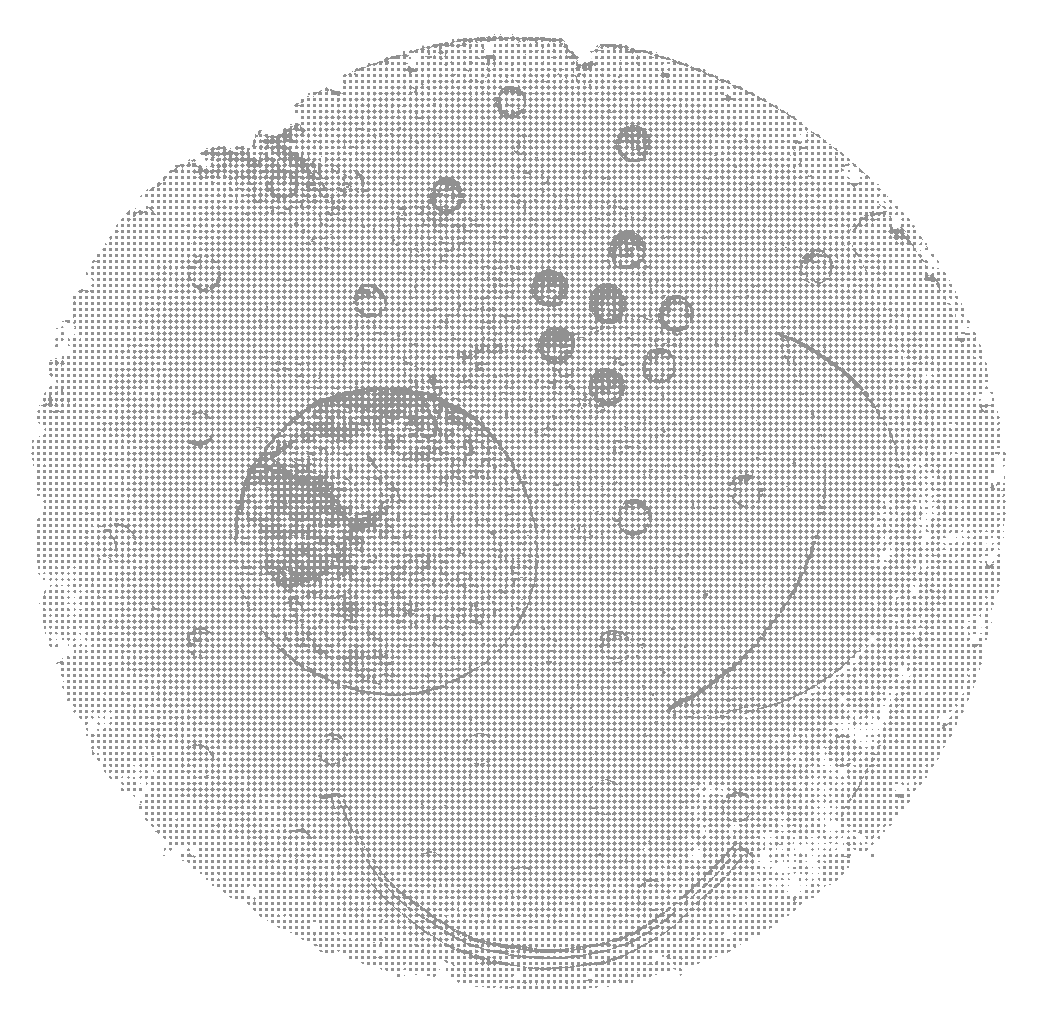
\includegraphics[width=4.5in]{images/0_00-Cover.png}\\[10ex]
            {\erhao \bfseries  \@title }\\[50ex]
            {\sanhao  \@author}\\[5ex]
            {\sihao \monthyeardate\today}\\[1ex]
        \end{center}
    \end{titlepage}
\makeatother
\thispagestyle{empty}
\newpage
%Add content for page two here (useful for two-sided printing)

\newpage
\thispagestyle{empty}
\maketitle
\begin{center}
    \ccbysa
\end{center}
\thispagestyle{empty}

\newpage

\setlength{\parindent}{0em}
\setlength{\parskip}{1em}

\chapter*{序言}

幼时夏夜,在屋顶乘凉,仰望壮丽的星空,时而会有一些遐想:在某个闪亮的星星附近,是否也有另一个“我”,同样在仰望星空,同样在发问?
后来读到 Ted Chiang 的《你一生的故事》,深为外星异质文化带来的观念冲击而着迷。为什么呢?因为人们可以通过不同来重新审视自己。

我们常常藏身于观念的硬壳里,很多观念创建已久,已经成为我们每个人思考的一部分;当我们说到它,仅仅一个熟知的词汇脱口而出,压根没想它真正的意义。
当重新尝试用观念创造者的角度来思考时,我们才恍然发现一个个想法的背后,对它们的思考并不是那么简单。不同会促使我们反省僵化的思维。

古时,庄子作出了一篇篇寓言,扬雄写了《太玄》与《法言》,这些著作或许有作者的深意;今人即使不认同这些背后的想法,但也不得不惊叹古人各种不同的瑰奇想象。
想象可以通过小说来表达,却重在情节而失之知识的严谨;知识可以通过严谨的论文来表述,可缺少了情趣与浪漫。

那么这本小书想达成什么呢?仅仅是想为成长中的青少年,开启一扇可以望见星空的窗,去感受外面无限的宇宙。这是笔者在写这本书时想到的,故以此为序。

\newpage

\setlength{\parindent}{0em}
\setlength{\parskip}{0em}

\renewcommand\contentsname{目录}
\tableofcontents
\thispagestyle{empty}

\newpage

\setcounter{page}{1} %Start the actually document on page 1

\setlength{\parindent}{0em}
\setlength{\parskip}{1em}

\chapter{人类对宇宙的认识之路}

\section{远古的探寻}

自古以来,天空中的日、月、星辰引发了人们无尽的想象和探究。1999 年人们在德国发现了内布拉星象盘,它是公元前 16 世纪青铜时代的器物。
在这个铜盘之上同时出现有太阳、月亮和星辰。根据一种解释,该盘上太阳和月亮之间的那团七星,是著名的金牛座“七姐妹”—昴宿星团。
内布拉星象盘(Nebra sky disk)艺术式地表现了人们对宇宙的思考与追寻。

\begin{figure}[ht]
\centering
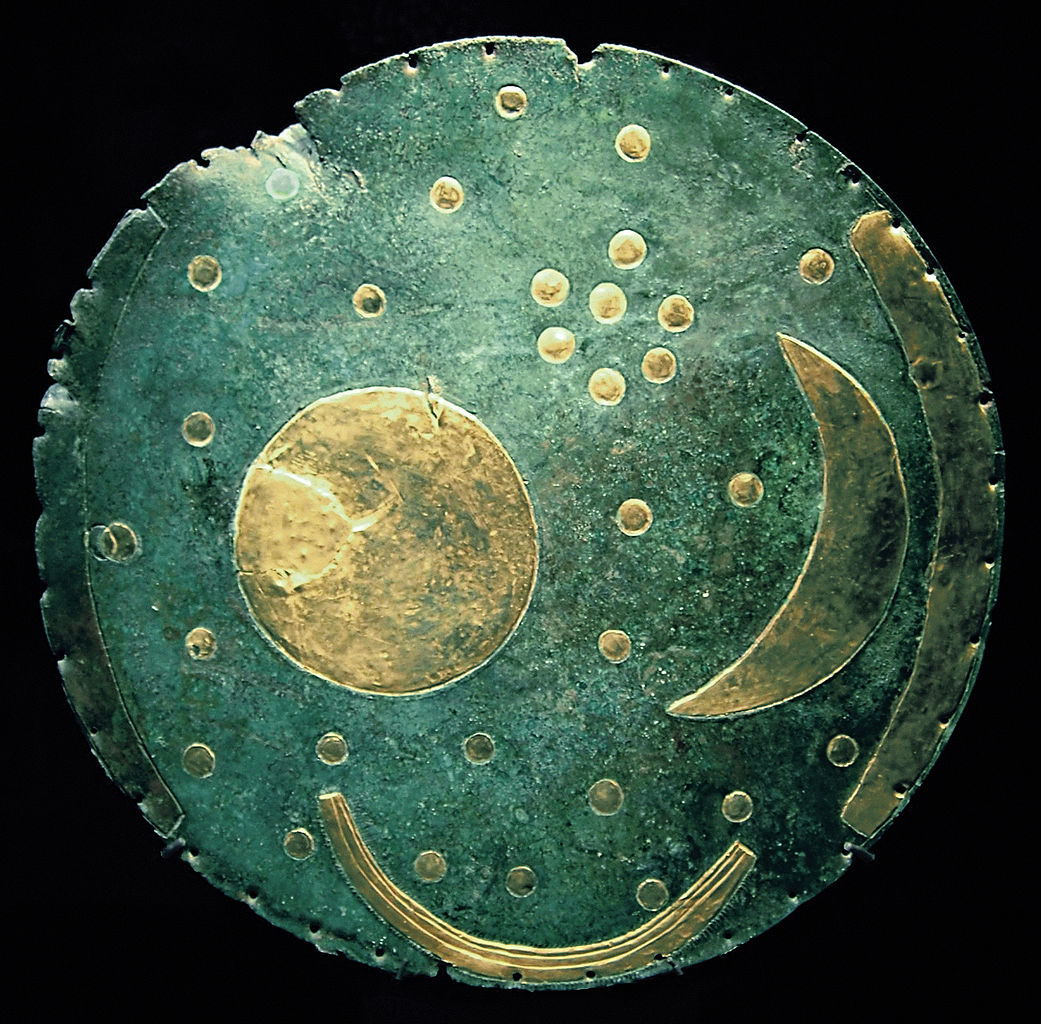
\includegraphics[width=2.5in]{images/1_01-Nebra_sky_disk.jpg}
\caption{内布拉星象盘(图片来自于维基共享资源计划)}
\end{figure}

然而人类对宇宙的追寻并不只停留在艺术式的表现,更在于能够精确预测天文现象。根据一种假说,建于公元前两、三千多年前的英国巨石阵(Stonehenge)
可以用来定位日月的位置并预测日食的发生。预测方法是使用巨石阵内 56 个奥布里洞(Aubrey holes)来实现的,它的原理是基于用公分子 56 来近似表达三个天文周期。

\begin{figure}[ht]
\centering
\includegraphics[width=5.0in]{images/1_02-Stonehenge.jpg}
\caption{巨石阵(图片来自于维基共享资源计划)}
\end{figure}

这三个天文周期分别是太阳的运动周期(地球的周年运动)、月球的运行周期和沙罗周期,它们的周期和近似的分数表示如下表所示。于是我们可以把沙盘的圆周等分
成 56 份,然后在上面简单地计数,来模拟日、地、月的运行。并且这些模拟可以不断通过观测来校正,这样使得整个预报系统能够长期相对精确地运行。

\begin{table}[tbhp]
\centering
\begin{tabular}{|c|c|c|c|}
\hline
天文现象 & 周期 & 近似周期 & 沙盘移动方法 \\
\hline
太阳的运行周期 & 365.26 天 & $ 56 \times \frac{13}{2} $ & 每 13 天移动 2 步 \\
\hline
月球的运行周期 & 27.32 天 & $ 56 \times \frac{1}{2} $  & 每天移动 2 步 \\
\hline
沙罗周期 & 18.61 年 & $ 56 \times \frac{1}{3} $  & 每年移动 3 步 \\
\hline
\end{tabular}
\caption{基于 56 的日食预测原理}
\end{table}

\section{文明时代}

在人类科学与技术史上,古希腊人制造的安提基特拉器械(Antikythera mechanism)无疑是古代的一个巅峰之作。它是古希腊人为了定位日、月和各大行星而设计制造的一个青铜器械。
该器械约在公元前 150 到 100 年之间被制造出来,迄今已有二千余年的历史。它的复杂的设计和制造,失传于历史长河之中,直到后世欧洲于 14 世纪制造出了天文钟后,才得以重现。

1900 年 10 月,安提基特拉器械在希腊安提基特拉岛海岸外的沉船中被发现,它随同大量的考古遗物和艺术品一起被打捞上来。1902 年考古学家在整理考古遗物时发现了它的特殊之处。
考古学家一开始认为这个器械是一种天文钟,但当时多数学者认为它太过复杂,远超同时期发现的其他物品,因此认为这里存在某种时代错乱,是后世的物品混进了这批考古遗物中。
直到 1951 年,英国物理学家德瑞克·约翰·德索拉·普莱斯(Derek J. de Solla Price)对该器械进行了系统性的研究,提出该器械通过齿轮组实现行星和恒星运动的模拟。其后科学家进行了多次系统的调查,进一步确认了普莱斯的观点。

\begin{figure}[ht]
\centering
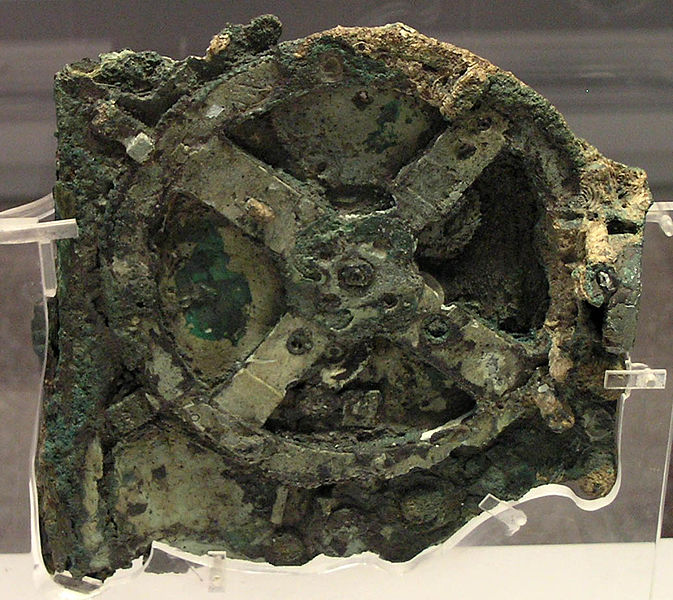
\includegraphics[width=2.5in]{images/1_03-Antikythera.jpg}
\caption{安提基特拉器械(图片来自于维基共享资源计划)}
\end{figure}

安提基特拉器械详细的 X 射线成像表明,它共有 37 个齿轮,能够模拟月球和太阳的运动、预测日食,甚至可以模拟月球的不规则运动。
在公元前 2 世纪,罗得岛的天文学家喜帕恰斯(Hipparchus)研究了这种运动,因此人们推测他可能参与了机器的制造。

在文献中,古代最重要的宇宙观来自于托勒密(Ptolemy)。

\section{文艺复兴}

尽管希腊人已经发展了多种不同的宇宙理论,但在古代很长时间里大多数人认为“地球是宇宙所有运动的中心”。这个命题赋予了地球无比特殊的地位。
然而即便是在中世纪也有人对此产生异议。

Nicole Oresme(132x? – 1382)是欧洲中世纪晚期的哲学家,他在神学著作中表达了上帝之下的众多不同世界的可能。

\begin{figure}[ht]
\centering
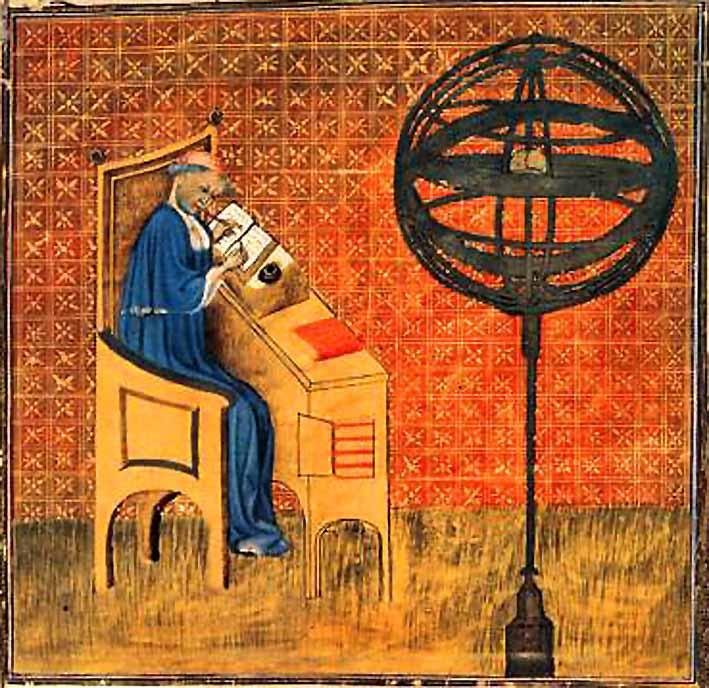
\includegraphics[width=1.5in]{images/1_02-Oresme.jpg}
\caption{Nicole Oresme(图片来自于维基共享资源计划)}
\end{figure}

\begin{figure}[ht]
\centering
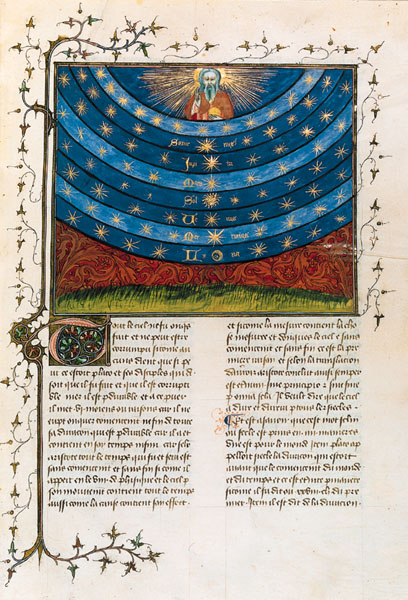
\includegraphics[width=1.5in]{images/1_03-Oresme_Spheres.jpg}
\caption{Nicole Oresme(图片来自于维基共享资源计划)}
\end{figure}

稍晚一些的 Nicholas of Cusa  (1401 – 1464) 也表达了类似的观点。

\begin{figure}[ht]
\centering
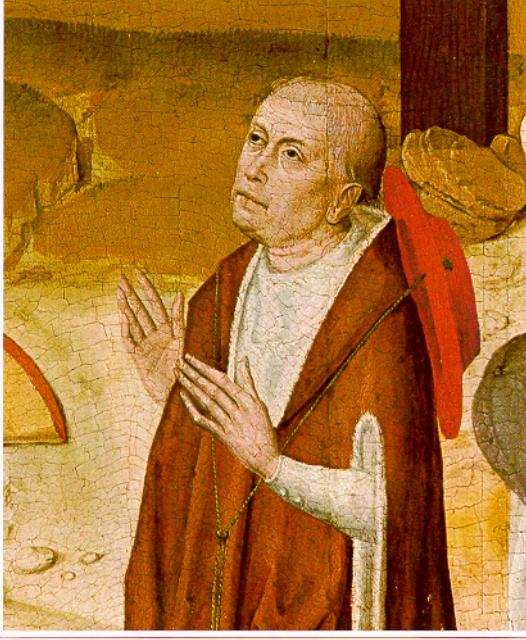
\includegraphics[width=1.5in]{images/1_04-Nicholas_of_Cusa.jpg}
\caption{Nicholas of Cusa(图片来自于维基共享资源计划)}
\end{figure}

欧洲进入文艺复兴之后,人才辈出。

Nicolaus Copernicus (1473 - 1543)

\begin{figure}[ht]
\centering
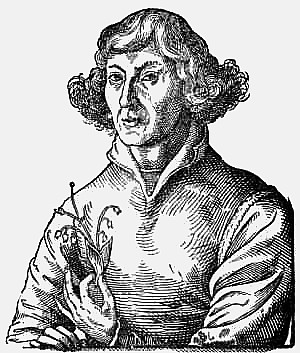
\includegraphics[width=1.5in]{images/1_05-Mikolaj_Kopernik.jpg}
\caption{哥白尼(图片来自于维基共享资源计划)}
\end{figure}

\begin{figure}[ht]
\centering
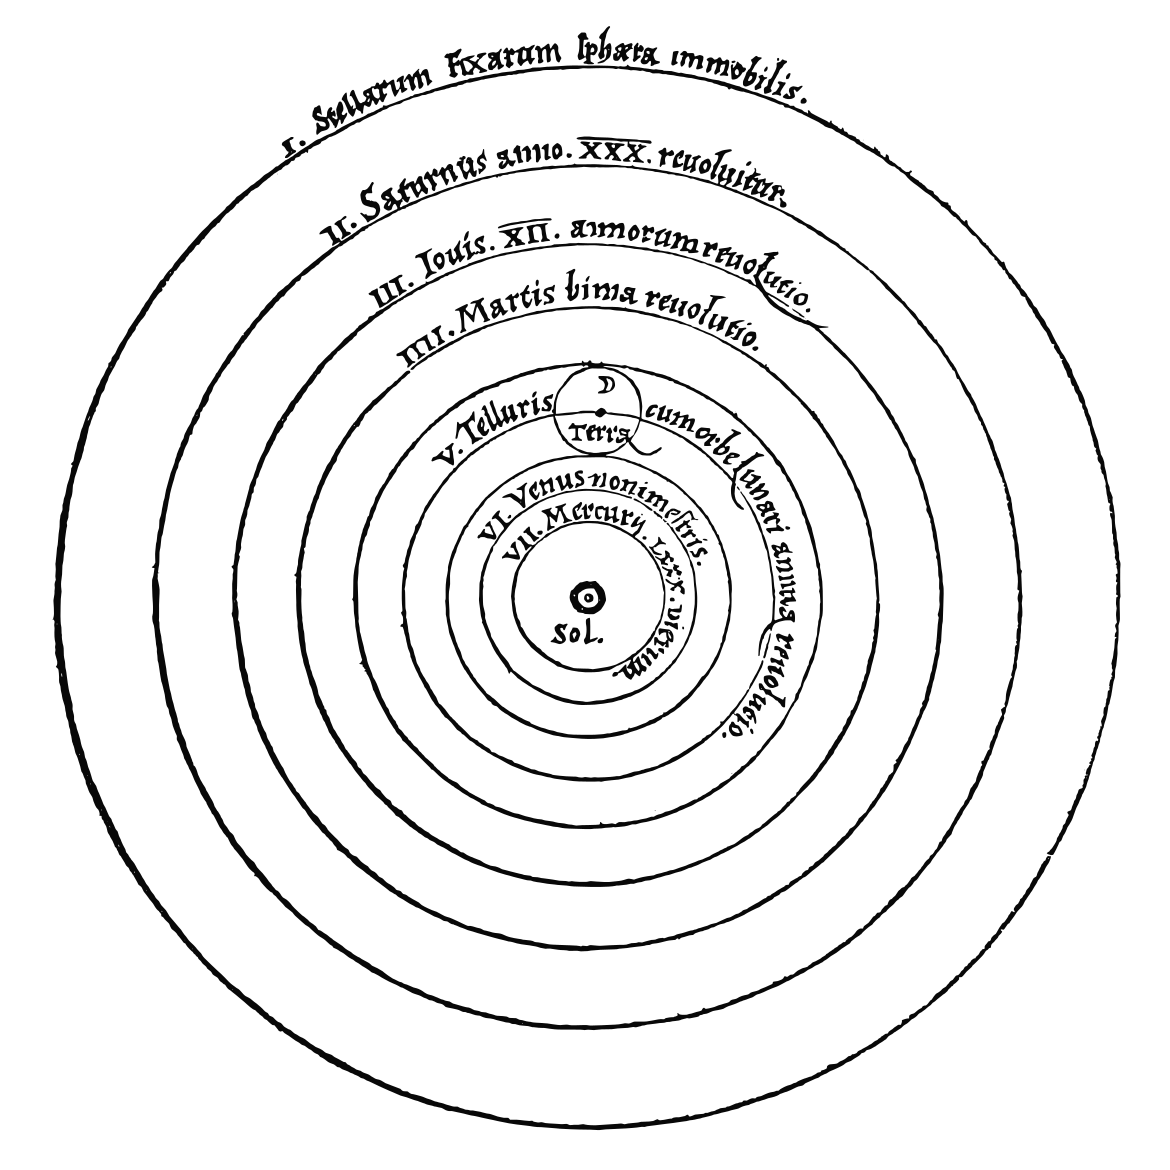
\includegraphics[width=1.5in]{images/1_06-Copernican_heliocentrism_theory_diagram.png}
\caption{《天体运行论》(图片来自于维基共享资源计划)}
\end{figure}

哥白尼在1543年去世之前,发表了著名的《天体运行论》,提出日心说,在《天体运行论》发表之后的几十年里,哥白尼的观点在欧洲不断传播。

Giordano Bruno (1548 – 1600)

布鲁诺因为他更为大胆的观点而付出了生命的代价。他认为宇宙无限,太阳是和其他恒星一样,所有恒星地位平等。

如今的罗马,在当年火刑的地点,伫立着一座布鲁诺的雕像。

\begin{figure}[ht]
\centering
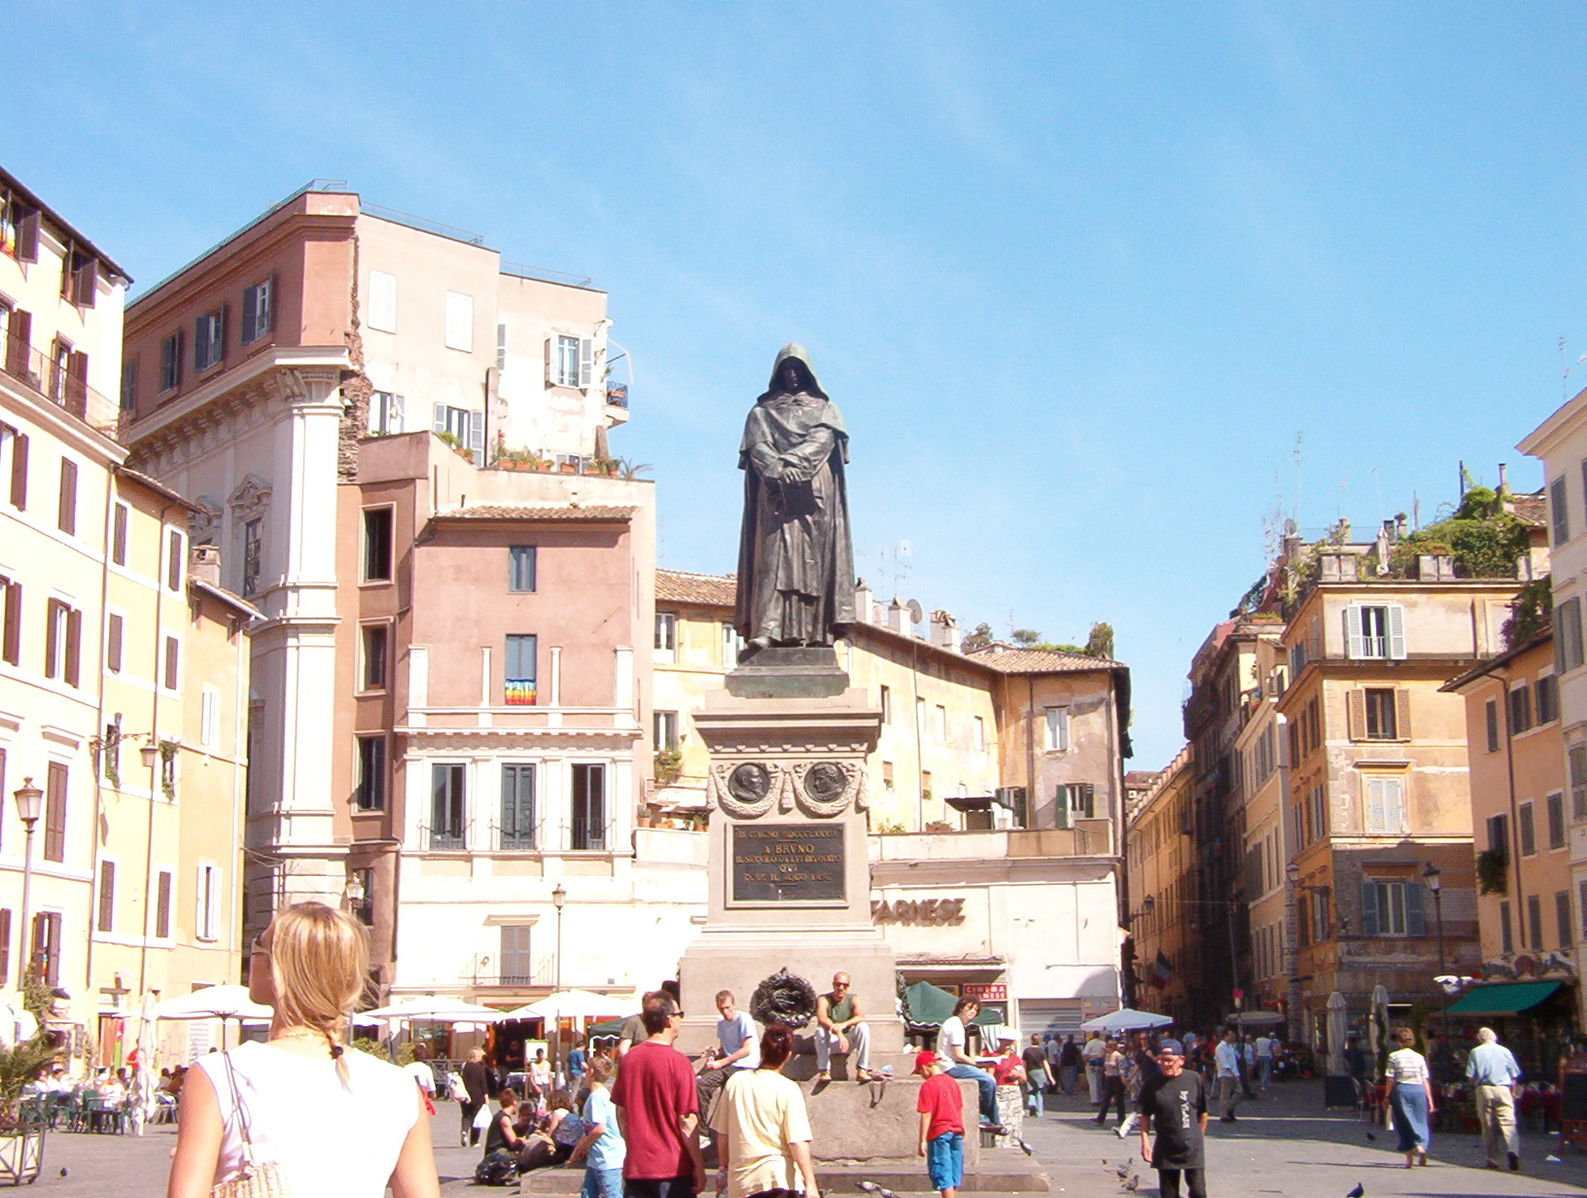
\includegraphics[width=1.5in]{images/1_07-Brunostatue.jpg}
\caption{布鲁诺像(图片来自于维基共享资源计划)}
\end{figure}

然而,在这些早期的日心说支持者中,最有贡献的是第谷。

\begin{figure}[ht]
\centering
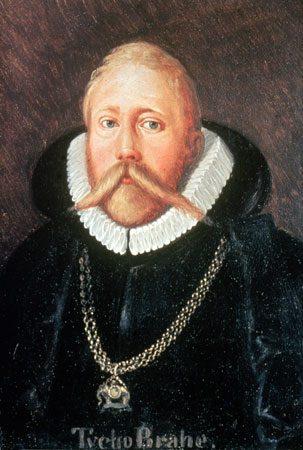
\includegraphics[width=1.5in]{images/1_08-Tycho_Brahe.jpg}
\caption{第谷(图片来自于维基共享资源计划)}
\end{figure}

Tycho Brahe (1546 – 1601)

第谷在天文学上的贡献,除了他的第谷体系之外,他还在汶岛(Hven Island)建立了天文台,从事大规模的天文观测。第谷的观测材料为他的学生开普勒的工作开辟了道路。

\begin{figure}[ht]
\centering
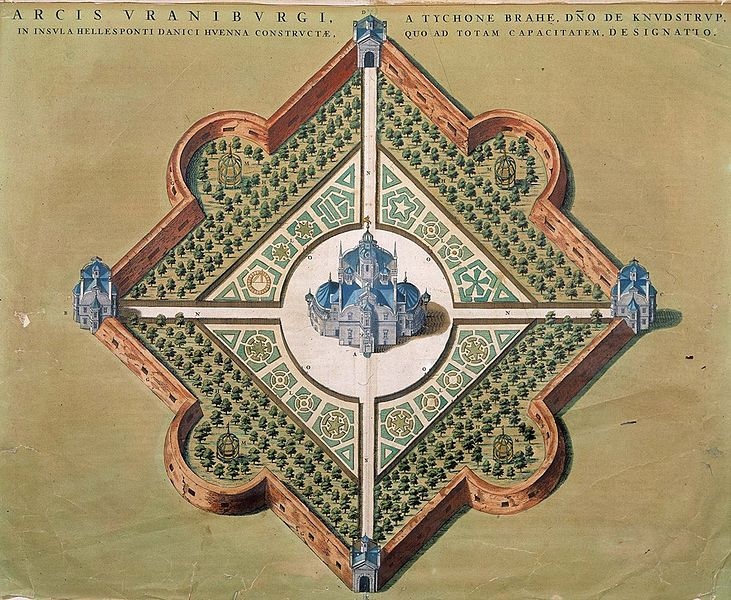
\includegraphics[width=1.5in]{images/1_09-Uraniborgskiss.jpg}
\caption{第谷建立的天文台(图片来自于维基共享资源计划)}
\end{figure}

\newpage

\section{近现代}

对自然深度的认识之路

开普勒建立了行星运动的三定律,开启了星体运动的数学描述之路。牛顿更进一步,发现万有引力的精确数学描述;在此基础上,拉格朗日、拉普拉斯、高斯、庞加莱建立了庞大的天体力学体系。物理学的革命:量子理论、相对论

对自然丰富的认识之路

威廉·赫歇尔(William Herschel)发现了天王星,同时他还对银河系形状建立了初步的认识。贝塞尔(Friedrich Bessel)第一次利用视差确定了太阳系到恒星天鹅座61的距离。

通过“沙普利-柯蒂斯之争”,人类确立了仙女座大星系的河外星系地位。

哈勃更利用造父变星确认河外星系的普遍存在。他还发现了河外星系的红移与距离的关系,也就是哈勃定律,为宇宙大爆炸理论提供了支持。宇宙微波背景噪音的观测。

系外行星

\newpage

\chapter{运动的星体}

最基本的问题有哪些?

星体间几何关系的变化导致的事件序列关系。

宜居性?

\section{运动方程}

下面我们先从星体的动力学方程开始讨论。我们指定两颗恒星的下标分别是1、2,行星的下标为,于是三个星体的质量分别是$m_1$、$m_2$、$m_3$,
位置分别是矢量 $\mathbf{x_1}$、$\mathbf{x_2}$、$\mathbf{x_3}$;因为行星质量 $m_3$ 远小于两个恒星的质量,可建立如下限定性三体问题的运动方程:

$$
\begin{cases}
\ddot{\mathbf{x_1}} = Gm_2r_{12}^{-2} \mathbf{e_{12}}\\
\ddot{\mathbf{x_2}} = Gm_1r_{21}^{-2} \mathbf{e_{21}}\\
\ddot{\mathbf{x_3}} = Gm_1r_{31}^{-2} \mathbf{e_{31}} + Gm_2r_{32}^{-2} \mathbf{e_{32}}
\end{cases}
$$

其中$r_{ij}$ 为星体 i 和 j 之间的距离,$\mathbf{e_{ij}}$ 为星体 i 和 j 之间的单位方向矢量。

\section{方程的解算}

三体系统很多情况下是不稳定的,常常会有一颗星体被抛射到无穷远处。
下图便是三体体系的一个著名例子—毕达哥拉斯三体问题的轨道演化图。两颗质量较大的星体相互围绕旋转下行,而质量最小的第三颗星体则被甩出,沿着双曲线上行。

毕达哥拉斯三体问题

我们问题的运动方程建立之后,便可以数值求解这个二阶常微分方程。理论上讲,我们忽略了行星的质量,会让系统的稳定性提高很多。
我们用最常用的数值求解方法—龙格库塔法[6]求解了该问题;但发现由于误差的积累效应, 整个体系不保持能量守恒;
于是,大多数情况下,三星体体系不稳定,行星会很快被抛出双星系。

这种不符合能量守恒的计算解中的能量变化,被称为能量漂移(Energy drift)。为了消除能量漂移,人们引入了辛方法来计算此类问题。
辛方法会保持系统的能量守恒。我们在这里则采用了一种二阶的辛方法 Verlet 积分。采用 Verlet 积分方法之后,我们就很容易计算出一条稳定的轨道了。

\section{天球系统}

为了更好的陈述后面几节,我们将讨论天球系统,我们以地球的天球系统为基础展开讨论。

天球是一个假想的以行星地心为球心的几何球面,行星自转导致恒星(母星和背景星空)在天球上有以天为单位的周日运动,
行星的公转导致恒星在天球上有以年为单位的周年运动。

地球天球的示意图

地球上天球的主要几何元素包括:

南、北天极:它们的指向长时间稳定
赤道面:以极轴为法线的大圆面
黄道面:本系统恒星周年运动所在的平面
黄赤交角:数值上等同于行星的自转轨道倾角

以上几何元素在瓦克星上依然成立。不一样的地方在于,黄道上有两颗母星沿着它运动。和地球类似,恒星的周日运动依然存在 ;但周年运动则大相径庭,
两颗母星的周年运动轨迹比较复杂,我们在后面章节仅作简单讨论,更多结果有待进一步研究。

\section{宜居性}

我们以液态水的稳定存在作为行星的宜居条件,可以做如下最为粗略的估计。假设母星为黑体且表面温度分别为 $T_1$ 和 $T_2$ ,母星的半径分别为 $R_1$ 和 $R_2$,瓦克星的行星反照率为 $\alpha$,半径为 $R_3$ ,视瓦克星为黑体且表面温度为 $T_3$  ,可以建立如下方程:

$$\left ( 1 - \alpha \right ) \left(  \frac{4 \pi R_1^2 \sigma T_1^4} {4 \pi r_{13}^2} + \frac{4 \pi R_2^2 \sigma T_2^4} {4 \pi r_{23}^2} \right ) \pi R_3^2= 4 \pi R_3^2 \sigma T_3^4$$

化简即得:

$$T_3 = \left[ \frac{1}{4} \left( 1 - \alpha \right ) \left( \frac{R_1^2}{r_{13}^2} T_1^4 + \frac{R_2^2}{r_{23}^2} T_2^4 \right ) \right ]^{\frac{1}{4}}$$

对地球而言,$\alpha$ 取值在 0.3 附近。

考虑到大气层的温室效应,我们只要令 $T_3$ 保持在 0 附近即可。

虽然这里宜居条件的估计涉及行星表面的物理机制,但最终化简的公式里,只保留了一些纯几何量的简单对比。所以,我们仍然把宜居问题的粗略估计纳入到恒星系建模的范围里。

\section{四方位}

方位感是人类内在生物机制。可是空间上的秩序并非空间自有的属性,是人类叠加到物理世界上的。可以说四方位、地名的概念是人类发明的最早的增强现实(Augmented Reality)的技术了。

从苏州地区的夜间卫星地图中的灯光可以看出,城市的街道格局是沿着东、西、南、北四个方向展开的。这其中的原因是因为在温带房子南北布局才能充分获得阳光。

\begin{figure}[ht]
\centering
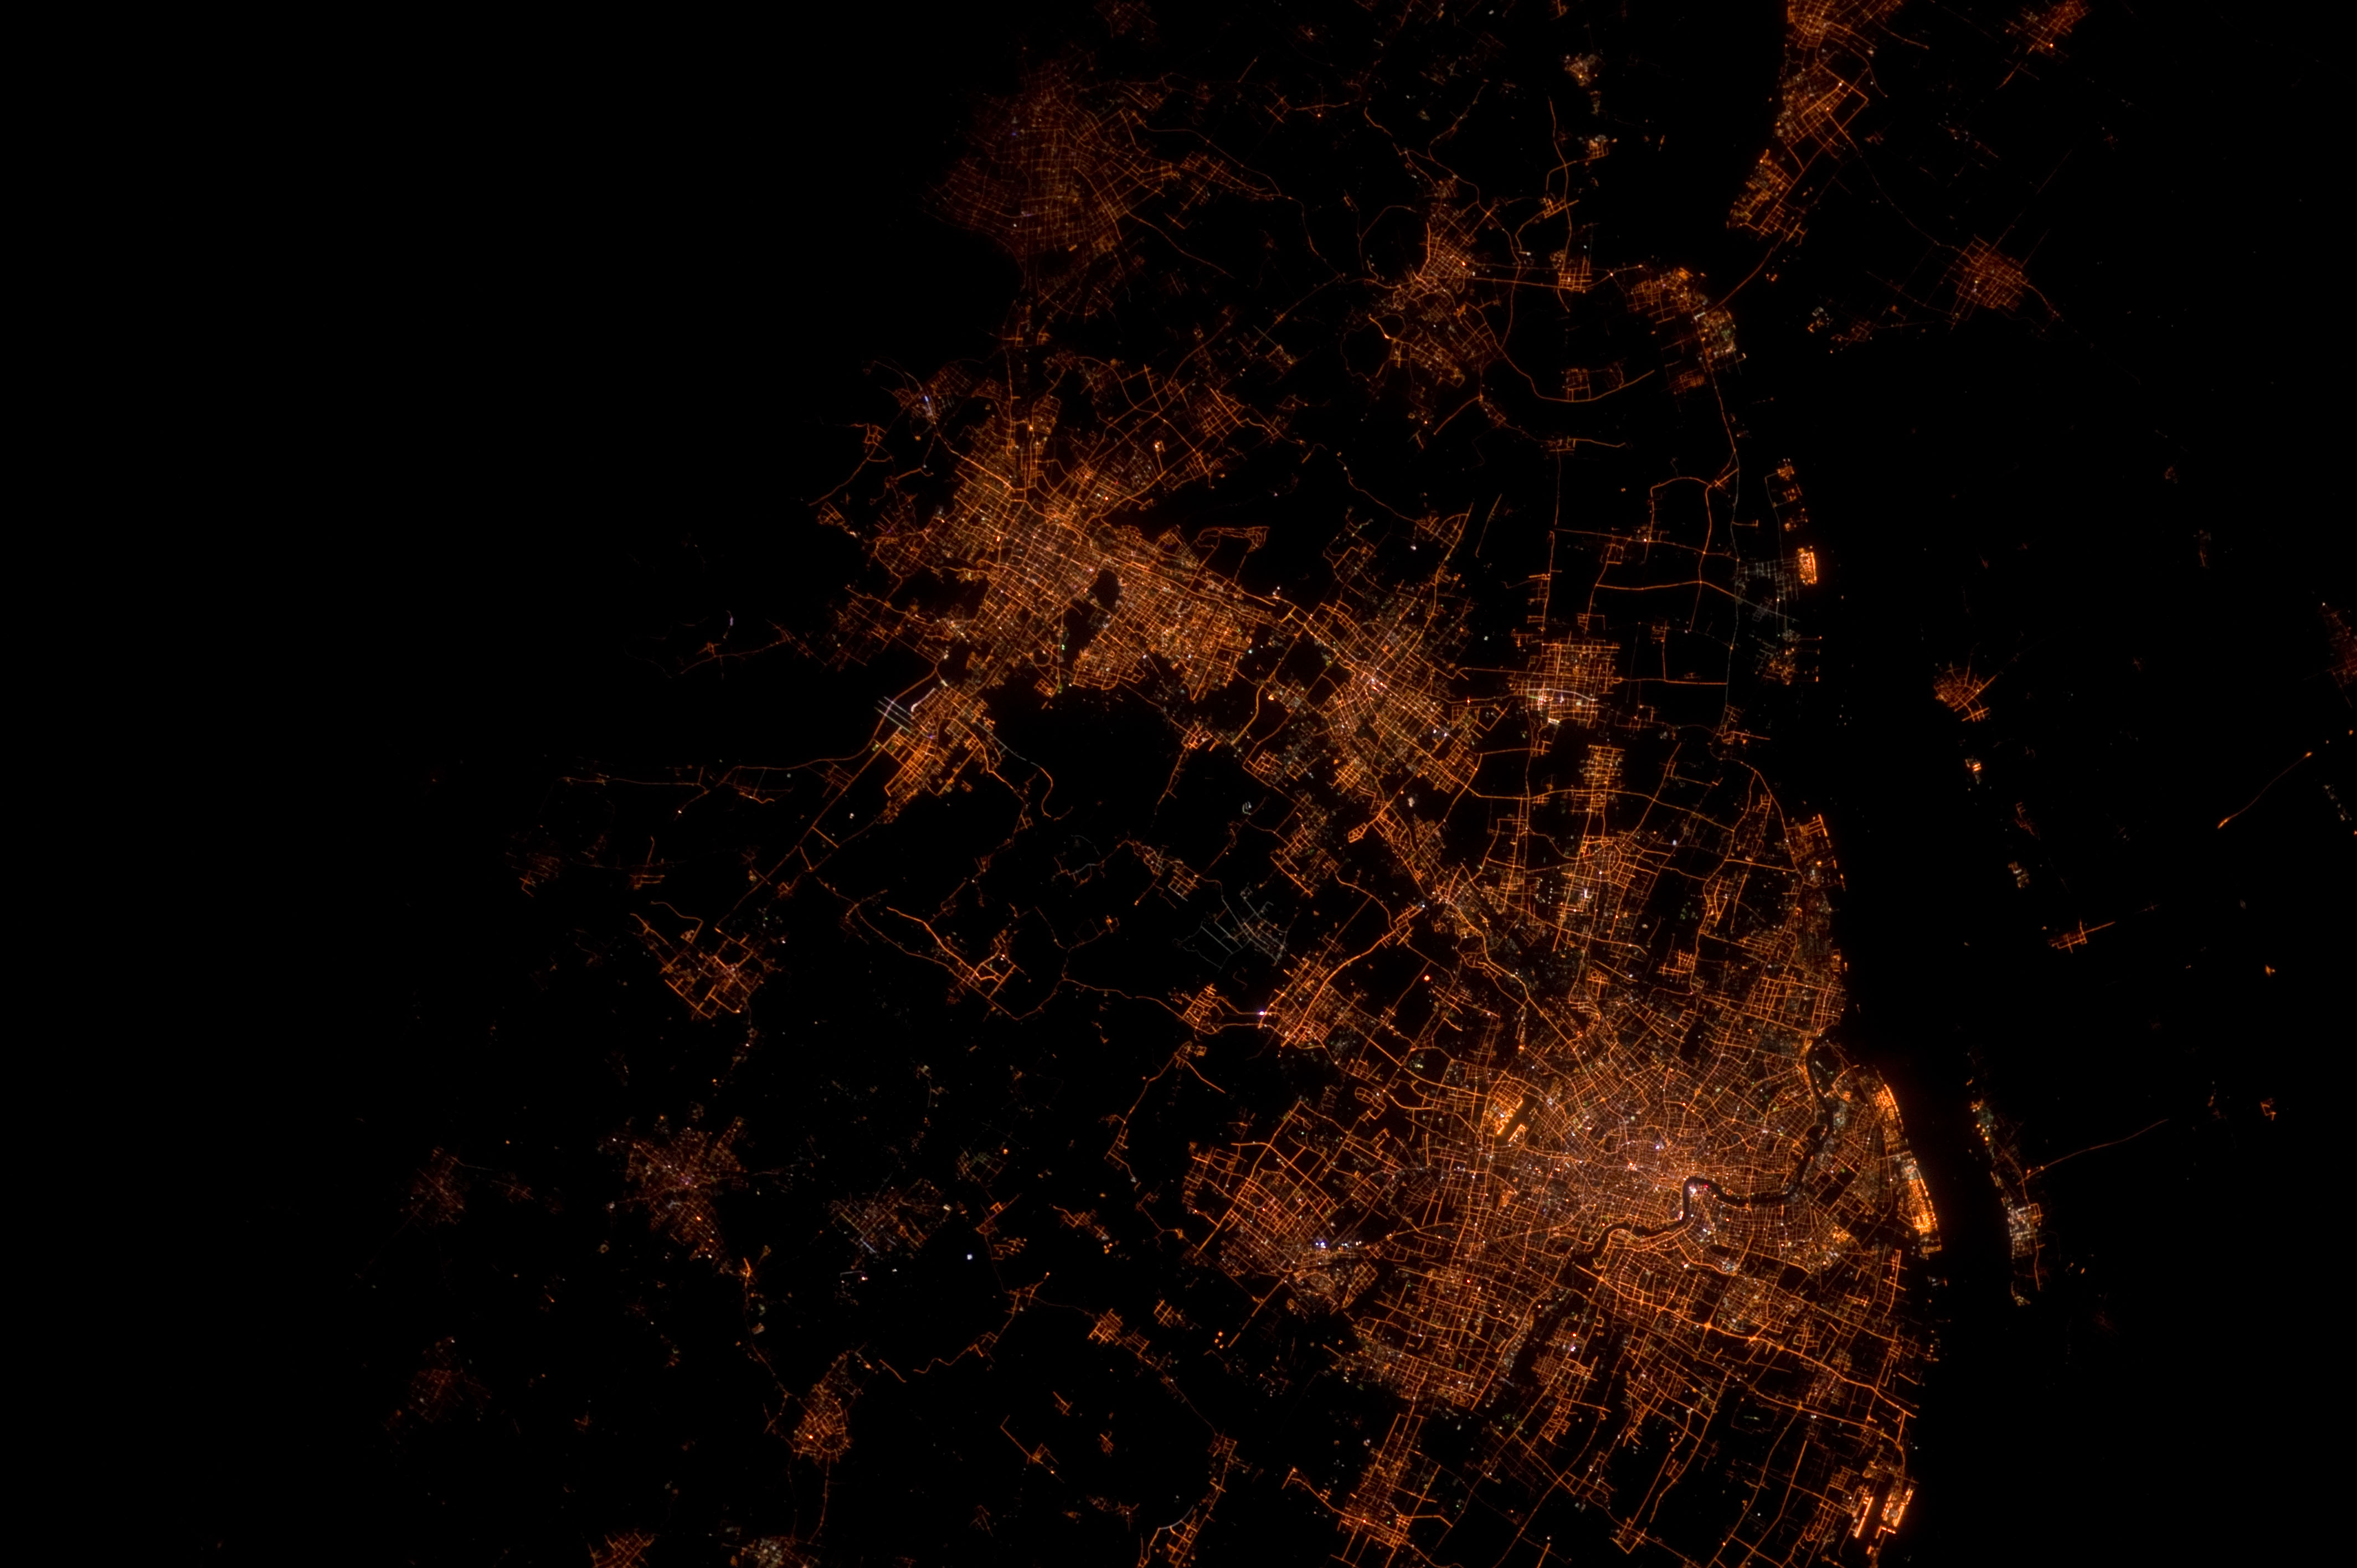
\includegraphics[width=1.5in]{images/4_01-ISS-30_Nighttime_view_of_Shanghai.jpg}
\caption{国际空间站拍摄的城市夜景(图片来自于维基共享资源计划)}
\end{figure}

可以说,太阳的光和热深深的渗透到我们文化的底层。在我们的大多数文化里,东、西、南、北四个方位是在儿童时期便教育给下一代的基本概念,
我们会借助于太阳东升西落或者房屋、街道的布局来表达它们。然而,仔细考究四方的严格定义,必须得对日月星辰的运行有透彻的理解才可以。
而因为这些基本概念潜入、物化在我们文化的各处,我们也往往忘记了这些基本概念的来源。瓦克星则给我们一个反思的机会。

当我从新思考瓦克星环境里的四方概念时,走了一段弯路,才意识到四方概念的本质。

东、西:地球上是太阳在春秋分东升西落的方位;然而瓦克星的春秋分的时间如何精确测定?
南:正午的太阳位置、立杆影子最短、太阳的光强最大的位置;然而有两个太阳,如何处理?
北:地球是北极星的位置;然而如果瓦克星没有北极星,那怎么测北?

似乎确定每个方向都会遇到一些问题。

我从南开始入手,写了数值模拟程序,看温带房子哪个方位布局才能最大获得阳光。我希望能看到一个不一样的结果,然而结果就是和地球一样的正南方。

由此,我才恍然大悟:自转轴相对保持恒定,这是四方概念成立的根源;所以,“北”是本质性的,其他三个概念都可以导出。

当然,瓦克星上还是有和地球不一样的地方。

比如,和四方联系的分至四时,在地球上会和昼夜平分、极昼、极夜现象联系起来。我们考察瓦克星时发现了一个奇特现象—双极昼现象。

\begin{figure}[ht]
\centering
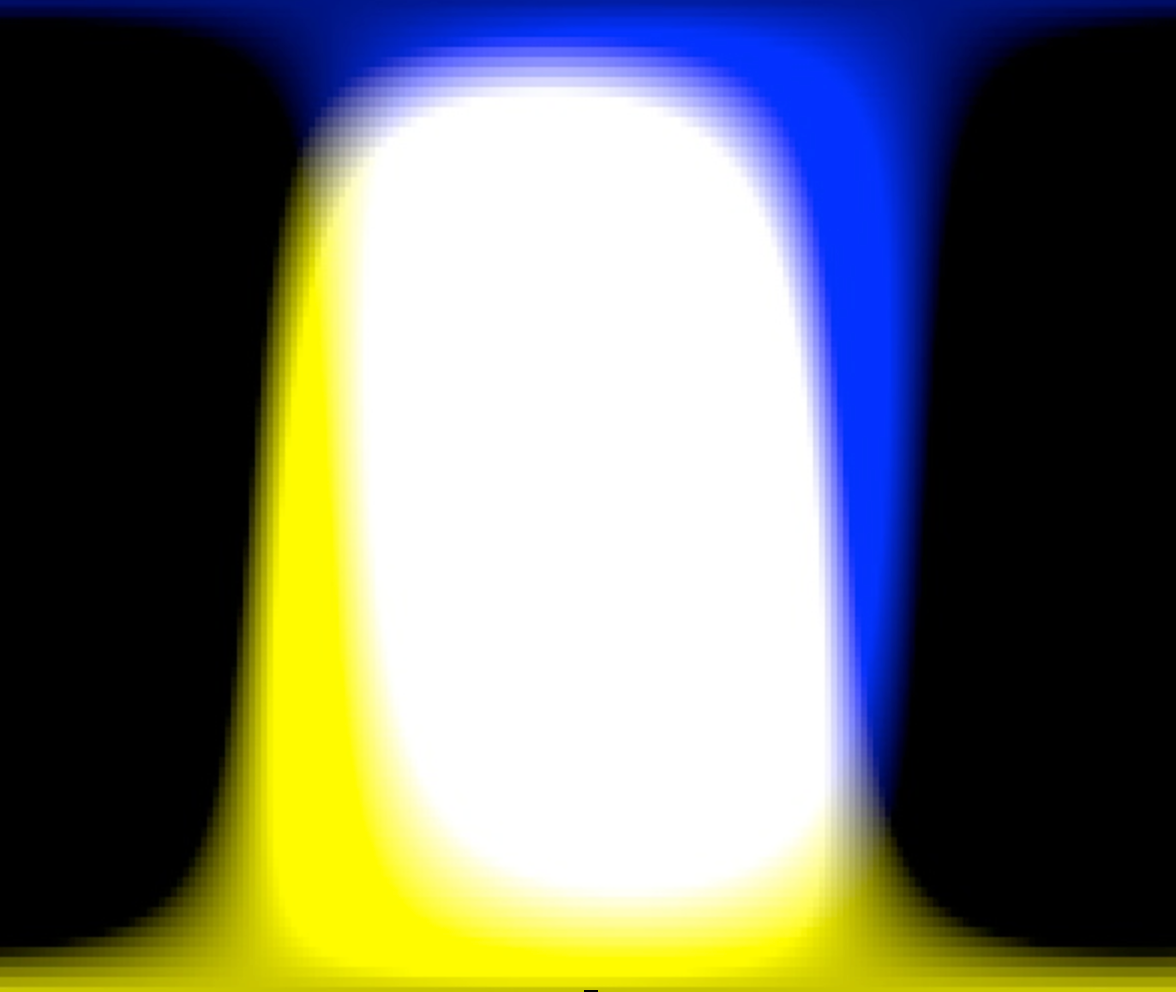
\includegraphics[width=1.5in]{images/4_02-day-night.png}
\caption{瓦克星上的双极昼现象}
\end{figure}

我们可以清楚看到,瓦克星南北两极都处于极昼。

\section{昼夜晨昏}

昼夜现象是由三颗星体和行星的旋转轴之间的相对几何关系确定的。容易想见在行星的球体表面上,每一个母星都对应一个昼夜变更的大圆 ,
它们对应圆面   和   的法线方向分别是    和   。 容易看出   是黄道面   的法线。

对比于昼夜现象的时间周期,我们可以不考虑岁差现象[11], 如同地球上的北极指向长期保持在北极星附近, 瓦克星的旋转轴  也是长期相对稳定的。
赤道面   的法线就是旋转轴  。

将以上关系编程就可以很容易模拟出瓦克星上的昼夜现象。那么瓦克星上的昼夜现象有什么特别的吗? 通过模拟我们发现,一年中会有短暂的几天时间,
瓦克星的南北两极同时处于极昼之中。这和地球大相径庭,地球上南极处于极昼,则北极处于极夜,或者反之。

\section{年}

正东、正西方位可以从正南、正北方位推导出来。但在地球上与此有关的概念还包括分至四时—春分、夏至、秋分、冬至;
在地球的各大文化里,这四个时间点往往有重要的天文与文化含义。

在春秋分点, 全球昼夜平分,太阳从正东升起、正西落下,太阳直射赤道;在夏至点,北半球那一天白昼时间最长,太阳升起和落下点位置最偏北,
中午立杆的影子最短,太阳直射南回归线; 冬至点则有类似的对偶现象。

那么瓦克星上会怎么样呢?容易理解的一点是,大多数周期性不再简单保持了。但更加透彻的理解这类问题,需要我们完整建立瓦克星的天球系统。
天球系统以背景星空为基准,然后确定各个星体在天球上的运动方式。当特定的几何关系出现时,就发生一定的天文事件。我们简单罗列一些容易观察到的事件:

母星沿着黄道运动到黄赤交点,此时母星直射赤道、正东正西起落,昼夜平分
某个母星对应白昼时间最长的正午时间点,此时这个母星直射某条回归线,中午立杆的影子全年最短。
两个母星的视夹角为0的点,此时发生食变
两个母星的视夹角最大

所以这里有一个重要的理论问题—确定星体间的这些几何关系发生的先后关系和周期。

\chapter{再造行星世界}

行星建模是涉及行星表面物理机制的建模过程。我们完成了地表特征的生成、估计温室效应和对大气现象的初步模拟。

最基本的问题有哪些?

大地的形态?潮汐?

大气各参量的极值?扰动形成的几何纹样?几何纹样的破坏与建立?洋流?

季节?

\section{大陆与海洋}

菱形方块算法[18]是常用的地表特征生成算法,它的常见形式是在一个方形区域上展开的。我们对它稍加变形,让它适应球面上地表特征生成的特殊需求。

如下图,标准的菱形方块算法反复执行如下两个大的步骤。


菱形方块算法的中心点生成

方块步骤:

取方块四角点的平均值作为中心点的基础值
再在基础值上叠加一个反映粗糙度的随机值,该随机值与方块边长和粗糙度正相关

菱形步骤:

取菱形四角点的平均值作为中心点的基础值
再在基础值上叠加一个反映粗糙度的随机值,该随机值与菱形边长和粗糙度正相关

两个步骤交错执行,会逐渐把方形区域密分填满。

我们在球面经纬网格基础上改造钻石方块算法,主要有四个要点:

最左经线和最右经线要粘合在一起,其上的对应格点取相同值
最上的纬线是北极点,要粘合成一个点,该纬线上的格点取相同值
最下的纬线是南极点,要粘合成一个点,该纬线上的格点取相同值
不同纬线上格点的间隔长度不等,与纬度的余弦成正比

算法中基础值会叠加一个随机的粗糙量,但实际模拟中我们寻求的是一个固定的地表特征,怎么解决这个问题呢?其实,只要采用确定性的伪随机数生成器[19],
同时赋予生成器相同的种子(seed),就可以顺利解决问题。

下图就是我们生成出来的一幅瓦克星全球地形图。可以看到有两个大陆和两个大的岛屿。大陆上有山地、高原、平原等地形区别。
当把地图按照相应的经纬度投影到球面之上,我们便得到了本文图(一)的瓦克星全球的俯视图,加上恒星照射产生的白昼和黑夜便得到了图(二)中的景象。

\section{温室效应}

本节我们用一个简化模型来估计瓦克星的温室效应。一方面,我们不考虑地气系统的纬向差异,认为系统参量只是纬度的函数。另一方面,我们假设瓦克星类似于地球,有相同的地气系统辐射平衡模式[21]。


图(十)
地球地气系统能量收支平衡示意图,图片来源 于NASA

我们设定  和  代表地表温度和大气温度,它们都是纬度  和时间  的函数。   代表全球的平均大气温度。 和   分别代表母星一和二的入射短波辐射带来的能量。我们考虑下垫面[22]的物态变化,如是否结冰,它会影响反照率  和比热容  。

依据能量转移过程的不同,我们做如下讨论:

短波辐射的大气吸收:

短波辐射的地面吸收:

地面的长波辐射的发出:

大气长波辐射的发出:

长波辐射的大气吸收:

长波辐射的地面吸收:

地面和大气之间的热交换(热力泡和蒸发 ):

由于不同纬度带之间温度差异,会带来大气热交换;一般而言,同一纬度带会有能量流入和流出,其净差我们可以设为:

上述公式中的参量可以通过和地球一样的假定值来获得。联立前面诸公式有

我们可以根据本式展开模拟。


\section{气温的纬度分布}

\section{大气环流}

将基本的物理定律应用于大气的运动,我们可以得到大气运动基本方程[23]:



理论上,只要对上述基本运动方程差分化,我们可以直接应用最简单的欧拉法[24]来解算这个偏微分方程。我们这样做了,在经纬网格上展开了计算。在这个过程里遇到了一系列出乎意料但有意思的问题,这里我们仅举一个例子—极点问题。

在经纬网格里,极点被展成了90°纬线圈,从球面的一个内点转而变成了特殊的边界线。在解算偏微分方程时,我们需要引入什么样的边界条件才能表达极点的特殊性呢?

容易看到,对于极点上的标量  ,标量从一个点值变成经度  的函数:



对于极点上的一个长度为  沿着经度  指向极点的向量  ,该向量也应该变成经度  的向量函数  ,但该函数在经纬网格里应该取什么形式呢?假设向量  属于球面上的一个连续向量场  。对于极点附近的一个充分小的纬度圈 ,可以认为向量场  在整个小纬度圈上保持向量  不变,转换到经纬网格里有:



可以看到径线和纬线方向的分量值都和  的大小无关。我们可以认为极点的情况作为  的一种极限,采取和上式相同的形式。

我们的这个模拟在处理地面和大气的长波辐射方面还有一些缺陷,导致长期计算时系统发散,这些缺陷会在未来的计划里改进。这里只给大家展示我们的一部分模拟结果。


图(十一)
模拟开始时刻0度经圈气温沿着高度的分布状况



图(十二)
模拟一段时间之后0度经圈气温沿着高度的分布状况

上面两个图展示了,模拟开始和进行一段时间之后,气温沿着高度的分布状况。气温高的颜色是红色,气温低的颜色是蓝色。对比上面两个图可以发现,模拟开始时,地面长波辐射被近地大气层吸收,所以近地的气温高,而高空是冷的;然而系统演化一段时间之后,大气温度随着高度上升首先是出现逆变,高空中出现冷气层,渡过冷气层继续上升后,温度才开始上升。这恰巧和地球上的实际情况吻合,冷气层以下是对流层[25],冷气层以上是平流层[26]。

\section{海气耦合}

\section{理想大陆}

\section{季节}

\chapter{重建生物圈}

最基本的问题有哪些?

生命体的尺度与形态是什么样?
生命体基于什么机制运作?
是否有植物与动物的分野?
生命体之间有什么样的连接关系?
什么样的生态景观?

\section{生命与演化}

\section{尺度的大小}

我们先回顾地球生物的异速生长现象。异速生长律是实际测量到的一类幂率关系,
它把生物体的尺度同其生理、生态特征联系起来。而这个观测到的幂率,往往不同于将生命体几何结构同构扩张后得到的理论幂率,故此称为异速生长。

文献中经常提到的异速生长现象包括:

体重和摄食率正相关,幂率为 0.7。
体重和基础代谢率水平正相关,幂率为 0.75,称为克莱伯定律
体重与内禀增长率负相关,幂率大约在 -0.27 左右

我们其实可以把异速生长律理解为一种高效的编码方式,仅仅尺度一个参数就决定了生理学和生态学的很多特征。

形态学信息:对植物来说,可以包括L系统的生长规则;对动物来说可以包括特征尺度、骨架结构、体重等
行为学的信息:如最大奔跑速度
生态学信息:内禀增长率、食谱组成等

\section{植物形态}

\section{动物形态}

\section{生态带}

\chapter{另辟蹊径的文明}

最基本的问题有哪些?

数制、逻辑是否是普遍的?

语言:基础词汇、语法范畴的人类学考察?

文字:几何形态的考察?

\section{数制}

大约在 18000 ~ 20000 BC 的 Ishango 骨刻,是目前人们发现的最早和数目有关的考古实物,它处在刻痕记事的阶段。
如果不考虑实物的形态,仅从抽象角度看,在这个阶段人们采用符号 1 的累记来表示更大的数目。
这种方式在表示形式上极为繁赘,尤其对大的数目,几乎不具有实际的可行性。但凭借这种简单的记号,人们有了对数目概念的理解。

\begin{figure}[ht]
\centering
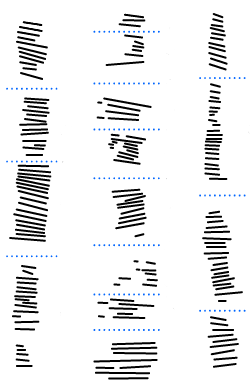
\includegraphics[width=1.5in]{images/IshangoAllColumns.png}
\caption{Ishango 骨刻(图片来自于维基共享资源计划)}
\end{figure}

在这个阶段,人们可以通过分堆的方法进行乘法运算。但这种方法仅仅限于小数目之间的乘法。

\begin{table}[tbhp]
\centering
\begin{tabular}{|c|c|c|c|c|}
\hline
\specialcell{ \ding{108} \\ \ding{108}\ding{108} } &
\specialcell{ \ding{108} \\ \ding{108}\ding{108} } &
\specialcell{ \ding{108} \\ \ding{108}\ding{108} } &
\specialcell{ \ding{108} \\ \ding{108}\ding{108} } &
\specialcell{ \ding{108} \\ \ding{108}\ding{108} } \\
\hline
\end{tabular}
\caption{计算 3 与 5 的乘积}
\end{table}

人类进入文明以后,有了对抽象符号更强的操作能力。在古埃及,人们发明了另外一种复杂的计数体系,它能表示整数、分数和相关运算。
我们这里仅仅简单展示整数的表示和乘法运算。

\begin{table}[tbhp]
\centering
\begin{tabular}{|c|ccccccc|}
\hline
数值 & 一 & 十 & 百 & 千 & 万 & 十万 & 百万 \\
符号 & \pmglyph{\Hone} & \pmglyph{\Hten} & \pmglyph{\Hhundred} & \pmglyph{\Hthousand} & \pmglyph{\HXthousand} & \pmglyph{\HCthousand} & \pmglyph{\Hmillion} \\
描述 & 单竖线 & 踵骨 & 绳圈 & 水莲 & 屈指 & 蝌蚪 & Heh 神\\
\hline
\end{tabular}
\caption{古埃及象形文字里的整数符号}
\end{table}

组合上述的基本符号,古埃及人可以表达一些相对较大的整数。但古埃及人组合这些符号的方式,并没有非常严格的方法:
既可以从左向右,也可以从右向左,有时也会竖写。除此以外,古埃及人做乘法的方式,更加显示出他们的数制还处于一种早期形态。
下图展示了古埃及人如何计算 11 与 35 乘积的过程。

\begin{figure}[ht]
\centering
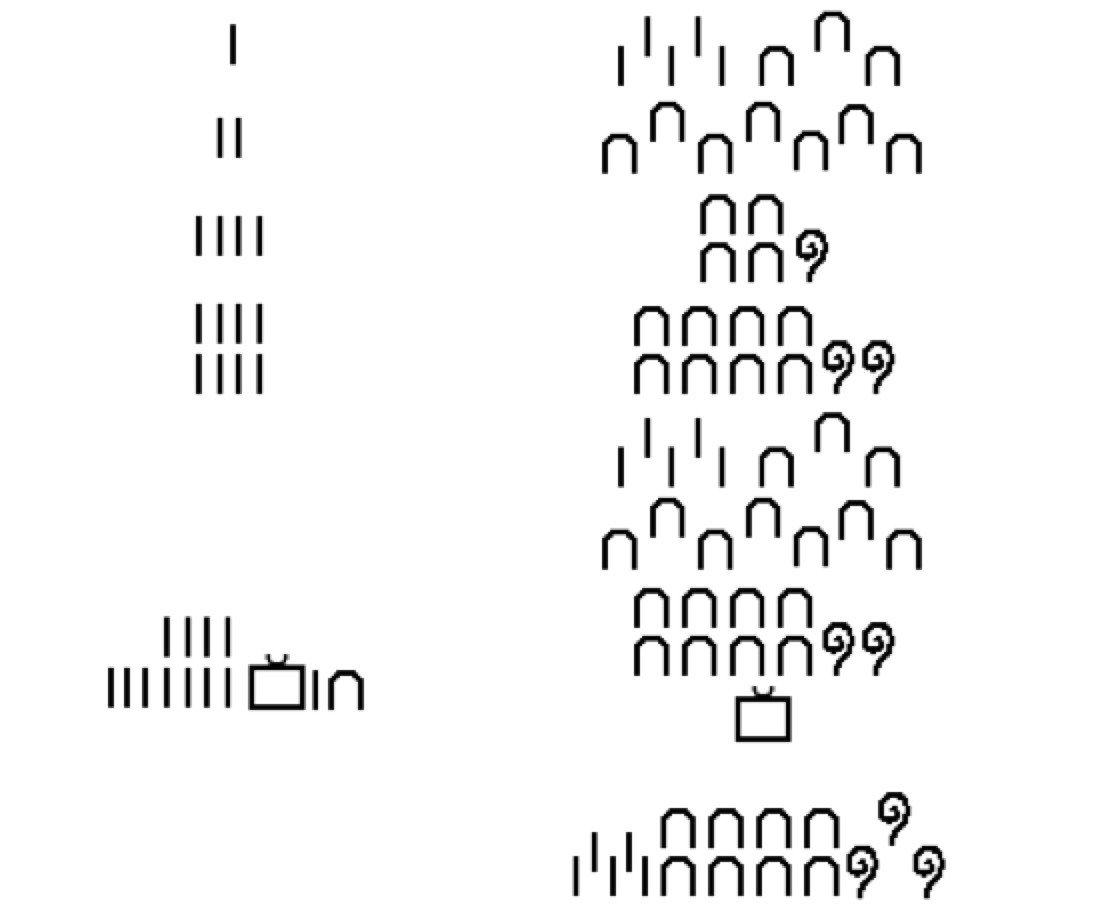
\includegraphics[width=3.5in]{images/ancient_egypt_multiplication.jpg}
\caption{计算 11 与 35 乘积}
\end{figure}

在这种方法里,首先构造 2 的幂的序列1、2、4、8……,同时 35 也按照 2 倍的关系相应扩大。
然后可以看出,11 能被分解成为了 1、2、8 的和,所以只要把 35 倍数里的 35、70、280 累加就可以得到结果。

但是数制的更加成熟的形态是数位制。在许多古文明中,数位制都被发明出来,如古巴比伦的 60 进制系统、古印第安文明的 20 进制系统。
对于乘法运算,中国古代很早就发明了九九乘法表,清华简中的“算表”作为考古实物依据,把发明年代至少向前推进到战国时代。
十进数位制和九九乘法表结合在一起,人们能够完整的表达所有自然数,并计算任意自然数的乘法。
当今,阿拉伯数字符号、十进数位制、九九乘法表都作为基础教育的内容,成为全人类分享的文明成果。

\begin{table}[tbhp]
\centering
\begin{tabular}{cccccccccccccccccccccccccccccccccccc}
  &   &   &   &   &   &   &   & 2 & 3 & 9 & 5 & 8 & 2 & 3 & 3\\
× &   &   &   &   &   &   &   &   &   &   &   & 5 & 8 & 3 & 0\\
\hline
  &   &   &   &   &   &   &   & 0 & 0 & 0 & 0 & 0 & 0 & 0 & 0\\
  &   &   &   &   &   &   & 7 & 1 & 8 & 7 & 4 & 6 & 9 & 9 &  \\
  &   &   &   &   & 1 & 9 & 1 & 6 & 6 & 5 & 8 & 6 & 4 &   &  \\
  &   & + &   & 1 & 1 & 9 & 7 & 9 & 1 & 1 & 6 & 5 &   &   &  \\
\hline
  &   &   &   & 1 & 3 & 9 & 6 & 7 & 6 & 4 & 9 & 8 & 3 & 9 & 0\\
\end{tabular}
\caption{竖式乘法的例子}
\end{table}

\section{历法}

历法是一种文化的计时方法,它也有服务于农业生产的目的。由此我们有天文历和农业历的分别;前者依据天文现象的周期性来计时,后者依据气候现象的周期性来指导农业生产。

地球上太阳的周年运动决定了地球的光热条件,进而决定了气候现象大的变化,因此,对于地球的许多文化,天文历和农业历是吻合的。那么瓦克星上会有什么不同呢?

基于我们的数值模拟,我们先考察一些现象的周期性:

恒星的周日视运动保持相对稳定的周期,因此天的概念会得到保持。
相对于背景星空,和行星公转相联系的周期是类周期的,因此年的概念需要修正。
行星上最显著的天文事件是两颗母星的食变,但该类事件是类周期的。
行星接收到的来自两颗母星的能量,有显著的年际变化,但存在一个以几年为跨度的类周期性。

因此,我们可以推测瓦克星的历法有如下几种类型:

星历:以背景星空为基准
食历:以两颗母星的食变为基准
农历:以气候周期为基准

这三种历法的基准都是类周期的,且周期各不相同,因此维护瓦克星的历法系统需要随时保持对各种星体的观测。
三种历法中,食历和农历的确立基准比较易于观测,因此容易被原始一些的文化建立;而星历的建立则复杂的多。

\section{逻辑}

\section{文字}

\chapter{余论}

\end{document}
